\section{Teilaufgabe 26}
\begin{aufgabe}
    Fügen Sie einen Anti-reset Windup hinzu und führen Sie noch einmal die 
    gleiche Simulationen durch (erkundigen Sie allein über Anti-reset Windup 
    wenn Sie nie davon gehört haben).
\end{aufgabe}
\begin{figure}[h!]
    \centering
    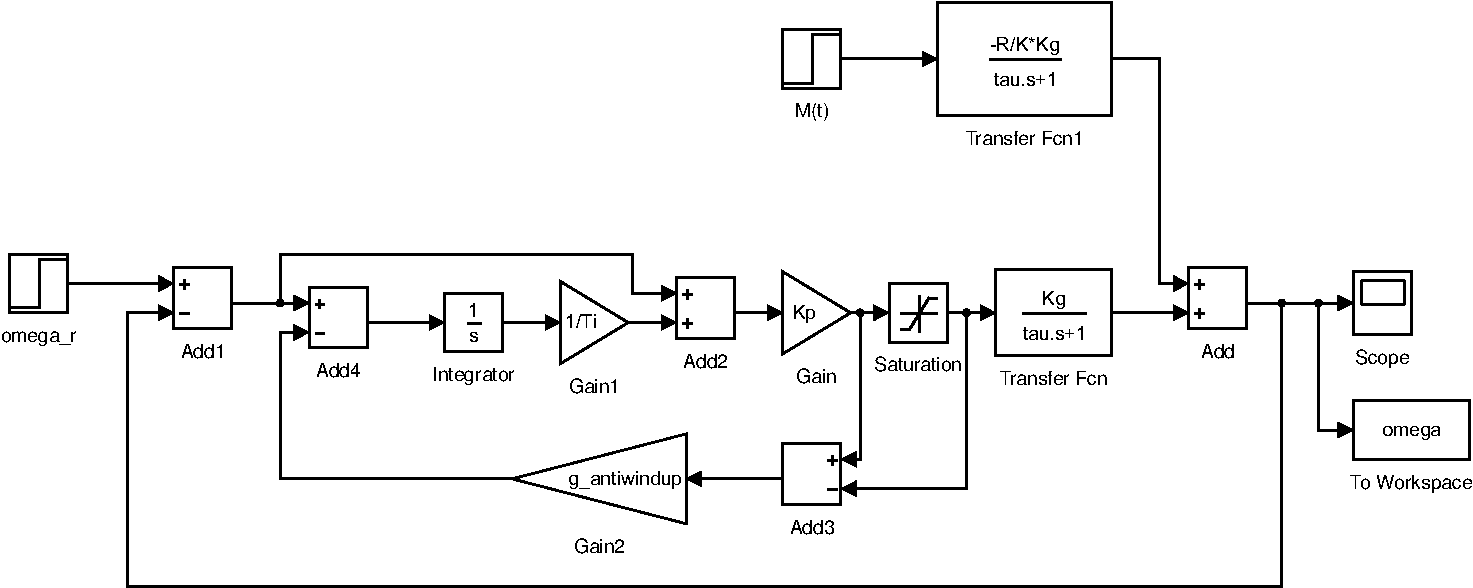
\includegraphics[width=0.6\textwidth]{26/regler_antiwindup.pdf}
    \caption{Regler in Simulink}
    \label{fig:26}
\end{figure}
\begin{figure}[h!]
    \centering
    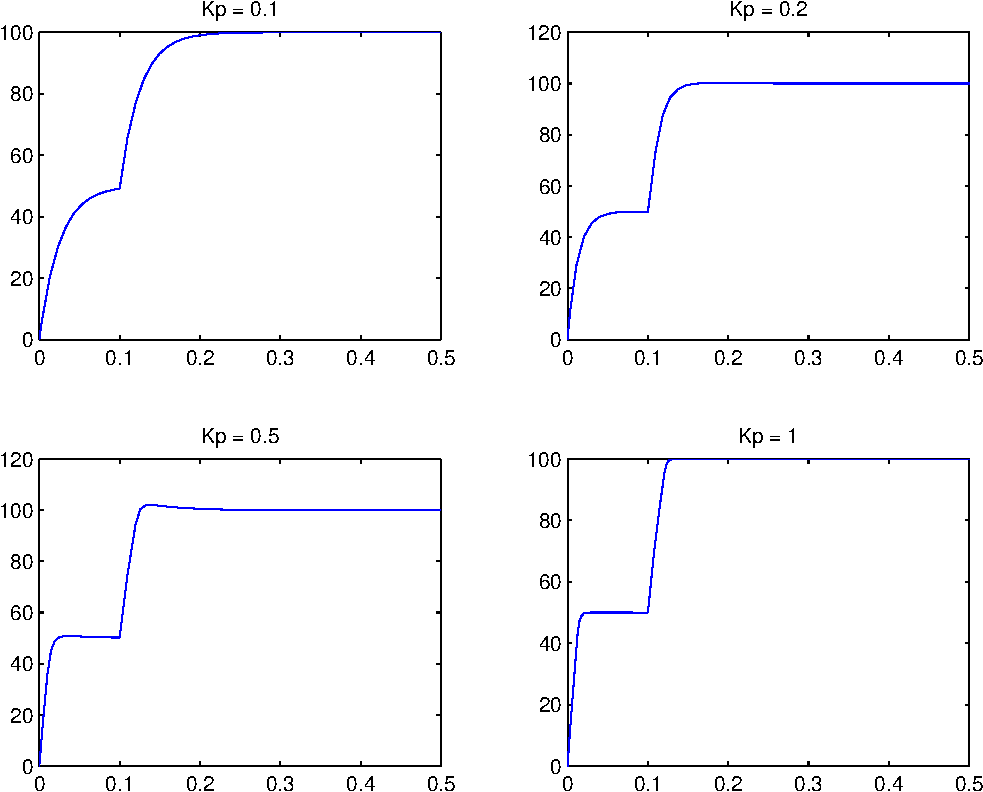
\includegraphics[width=0.6\textwidth]{26/regler_antiwindup_plot.pdf}
    \caption{Simulationsergebnis}
    \label{fig:26plot}
\end{figure}
